\newpage{\ } 
\thispagestyle{empty} 

\chapter{Materiales y Metodolog\'ia}
\lhead{Capítulo 4. \emph{Materiales y Metodolog\'ia}} % This is for the header on each page - perhaps a shortened title
En este cap\'itulo se describir\'an los materiales a utilizar en la elaboraci\'on de la metodolog\'ia, as\'i como tambi\'en aquellos a utilizar en las diversas pruebas y validaciones. Adem\'as se presentan las diversas características de las imágenes satelitales a ser empleados en el estudio. La metodolog\'ia nos presenta los diferentes procesos o m\'odulos necesarios para la estimaci\'on de p\'erdida de carbono.
\section{Materiales}
Un grupo de im\'agenes fueron utilizadas para los diferentes estudios y procedimientos de la metodologia, tales como:
\begin{itemize}
	\item Im\'agenes satelitales Landsat.
	\item Im\'agenes Campos Continuos de Vegetación (VCF).
	\item Im\'agen Mapa global de carbono - Paraguay.
	\item Paraguay Forest Change Product.
\end{itemize}
En el procesamiento e implementaci\'on de algoritmos fueron utilizados dos aplicaciones:
\begin{itemize}
	\item GRASS.
	\item Quantum GIS.
\end{itemize}
A continuaci\'on se hablaran con mayor detalle de los elementos citados.
\subsection{Im\'agenes}
En este apartado se pretende brindar las diferentes caracter\'isticas que presentan cada tipo de imagen utilizada en este trabajo..
\subsubsection{Landsat}\label{sec:landsat}
Landsat representa la colecci\'on m\'as larga y continua en el mundo de im\'agenes satelitales con resoluciones moderadas \cite{landsatNasa}. Cuatro d\'ecadas de im\'agenes proporciona un recurso \'unico para personas que trabajan en la agricultura, geolog\'ia, silvicultura, ordenaci\'on territorial, educaci\'on, cartograf\'ia e investigaci\'on del cambio global, como tambi\'en en respuesta de emergencias y operaciones de socorro.\\~\\
Las im\'agenes est\'an disponibles desde 1972 generados por una serie de 6 sat\'elites Landsat. Estos sat\'elites han sido un componente importante del Programa de Observaci\'on de la tierra perteneciente a la NASA, con tres sensores primarios evolucionando a lo largo de treinta años: MSS (Multi-spectral Scanner), TM (Thematic Mapper), y ETM+ (Enhanced Thematic Mapper Plus). 
El 11 de febrero del 2013 fue lanzado el Lansadt 8 correspondiendo al futuro de los sat\'elites Landsat con dos nuevo sensores, Operational Land Imager (OLI) y el Thermal Infrared Sensor (TIRS). La Tabla \ref{t:landsattipos} nos muestra las diferentes resoluciones de los sensores Landsat.

\begin{table}[htb!]
	\centering
	\begin{tabular}{|c|c|c|c|c|c|}
		\hline
		\multirow{2}{*}{\textbf{Landsat}} & \multicolumn{5}{c|}{\textbf{Resoluciones}}                                                             \\ \cline{2-6} 
		& \textbf{Espacial} & \textbf{Espectral} & \textbf{Radiom\'etrica} & \textbf{Temporal} & \textbf{Sensor} \\ \hline
		1                                 & 79x79 m2          & 5 bandas           & 6 bits                  & 18 dias           & MSS             \\ \hline
		2                                 & 79x79 m2          & 5 bandas           & 6 bits                  & 18 dias           & MSS             \\ \hline
		3                                 & 79x79 m2          & 5 bandas           & 6 bits                  & 18 dias           & MSS             \\ \hline
		4                                 & 30x30 m2          & 7 bandas           & 8 bits                  & 16 dias           & TM              \\ \hline
		5                                 & 30x30 m2          & 7 bandas           & 8 bits                  & 16 dias           & TM              \\ \hline
		6                                 & 30x30 m2          & 8 bandas           & 8 bits                  & 16 dias           & ETM+            \\ \hline
		7                                 & 30x30 m2          & 8 bandas           & 8 bits                  & 16 dias           & ETM+            \\ \hline
		8                                 & 30x30 m2          & 9 bandas           & 12 bits                 & 16 dias           & OLI/TIRS        \\ \hline
	\end{tabular}
	\caption{Resoluciones de los sat\'elites Landsat.}
		\label{t:landsattipos}
\end{table}
El Sistema de Referencia Mundial Landsat-2 (WRS-2: Landsat Worldwide Reference System-2) provee un esquema de indexaci\'on para el patr\'on de repetici\'on de la trayectoria orbital terrestre seguida por las plataformas espaciales Landsat 4, 5 y 7 sobre los 16 d\'ias de su repetitivo ciclo orbital \cite{els2015refere}. El original WRS (WRS-1) fue dise\~{n}ado para las misiones Landsat 1, 2, y 3, las cuales se movieron en una \'orbita m\'as alta. El actual WRS-2 fue dise\~{n}ado para la \'orbita a 705 Km usada para las \'ultimas misiones. En la Figura \ref{fig:wrs2Image} podemos observar los \'indices (Path y Row) en el momento de la obtenci\'on de una imagen satelital Landsat para una zona.

\begin{figure}[H]
	\centering
	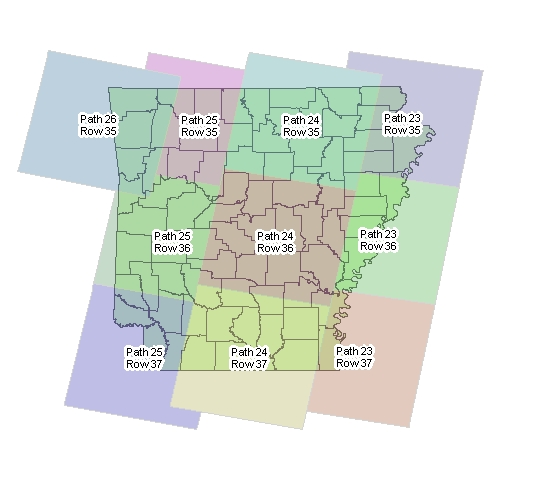
\includegraphics[width=0.8	\textwidth]{./Figures/cap4/wrs2_22.jpg}
	\caption{Ejemplo WRS-2 Path/Row}
	\label{fig:wrs2Image}
\end{figure}

El Servicio Geol\'ogico de los Estados Unidos (USGS) es una agencia cient\'ifica de los Estados Unidos, el cual proveen un producto llamado L1T (Level 1 Terrain Corrected) que implica las im\'agenes Landsat con datos pre-procesados para una correcci\'on radiom\'etrica sistem\'atica y correcci\'on geom\'etrica mediante la incorporaci\'on de puntos de control en tierra. Estos productos est\'an en la Web de forma gratuita \cite{landsatNasa}.


\subsubsection{Campos Continuos de Vegetación (VCF)}\label{sec:vcf}
Las im\'agenes VCF contienen estimaciones proporcionales para los tipos de cobertura vegetal: vegetaci\'on le\~{n}osa, vegetaci\'on herb\'acea y suelo desnudo. El producto se deriva de las siete bandas del sensor MODerate-resolution Imaging Spectroradiometer (MODIS) a bordo del sat\'elite Terra, perteneciente a la NASA. El esquema de clasificaci\'on continuo del VCF puede representar \'areas terrestres heterog\'eneas mejor que los esquemas tradicionales de clasificaci\'on discreta. Los sistemas de clasificaci\'on tradicionales indican donde se concentran los tipos de cobertura del suelo. El VCF posee un resoluci\'on espacial de 250x250 metros cuadrados y la colecci\'on de im\'agenes se encuentra disponible gratuitamente en la Web \cite{gl2015Uni}.
La Figura \ref{fig:vcfImage} nos presenta un imagen, con diferentes tonalidades de color, para los porcentajes de vegetaci\'on y los niveles digitales del agua como pixeles nulos.
\begin{figure}[H]
	\centering
	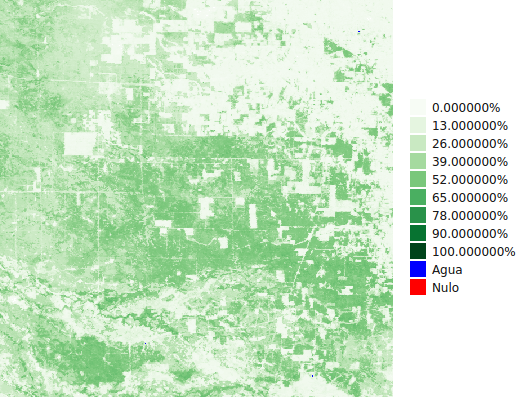
\includegraphics[width=0.8	\textwidth]{./Figures/cap4/vcf_image.png}
	\caption{Imagen VCF con diferentes tonalidades de color de acuerdo al porcentaje de vegetaci\'on.}
	\label{fig:vcfImage}
\end{figure}
\subsubsection{Mapa global de carbono - Paraguay}\label{sec:saatchiMapa}
El mapa global de carbono \cite{saatchi2011benchmark} nos provee la densidad de carbono, expresada en toneladas de carbono por hect\'area, del \'area ocupada por un pixel. En la actualidad existen diferentes mapas de carbono a nivel mundial \cite{saatchi2011benchmark}. La Figura \ref{fig:saatchi} representa el mapa global de carbono disponible para el Paraguay.
\begin{figure}[H]
	\centering
	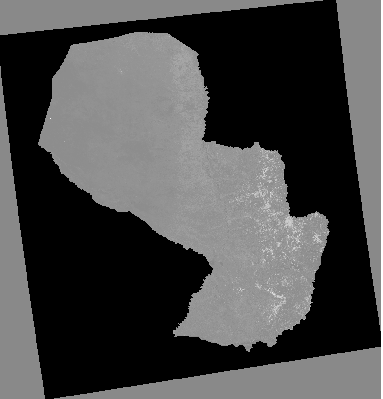
\includegraphics[width=0.8	\textwidth]{./Figures/cap5/saatchi.png}
	\caption{Mapa Global de Carbono - Paraguay}
	\label{fig:saatchi}
\end{figure}


\subsubsection{Paraguay Forest Change Product}\label{sec:fcc}
El Paraguay Forest Change Product (PFCP) muestra donde ocurri\'o la deforestaci\'on en Paraguay durante 1990-2000. El PFCP fue elaborado a partir de las im\'agenes Landsat TM y ETM+, identificando seis clases; bosque atl\'antico, Chaco bosques, el agua, no forestales y la deforestaci\'on. El producto puede ser utilizado para determinar procesos y patrones de cambio en la cubierta forestal. En la Figura \ref{fig:fcc} se puede observar el PFCP (disponible gratuitamente \cite{gl2015Uni}). En la Tabla \ref{t:pfcptab} se describe la representaci\'on de cada nivel digital en dicha imagen. .
\begin{table}[htbp]\centering
\begin{tabular}{|c|c|c|}
	\hline \textbf{Valor digital} &\textbf{ Representaci\'on} & \textbf{Color sugerido} \\ 
	\hline 1 & Bosque Atl\'antico & Verde \\ 
	\hline 2 & Bosque Chaque\~{n}o & Verde Claro \\ 
	\hline 3 & No Bosque & Agua \\ 
	\hline 4 & Agua & Azul \\ 
	\hline 5 & P\'erdida Bosque Atl\'antico & Rojo \\ 
	\hline 6 & P\'erdida Bosque Chaque\~{n}o & Purpura Claro \\ 
	\hline 
\end{tabular} 
\caption{Representaci\'on del valor digital en la imagen PFCP.}
\label{t:pfcptab}
\end{table}

\begin{figure}[H]
	\centering
	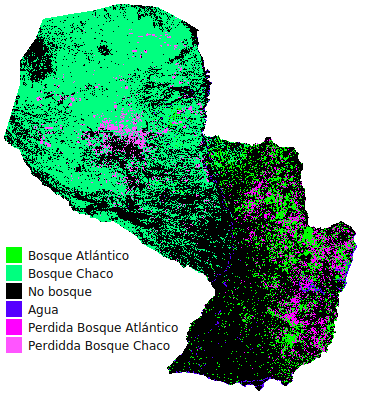
\includegraphics[width=0.7	\textwidth]{./Figures/cap4/fcc_paraguay.png}
	\caption{Paraguay Forest Change Product}
	\label{fig:fcc}
\end{figure}



\subsection{Aplicaciones}
Sistemas de informaci\'on geogr\'afica fueron utilizados para la manipulaci\'on de im\'agenes satelitales, como tambi\'en para dise\~{n}ar e implementar los algoritmos utilizados en la metodolog\'ia propuesta. A continuaci\'on se describen las aplicaciones utilizadas.

\begin{itemize}
	\item \textbf{GRASS: }es un software SIG  bajo licencia GPL (software libre) \cite{osgeoGrass}. El software soporta informaci\'on tanto raster como vectorial y posee herramientas de procesado digital de im\'agenes. Esta disponibles principalmente para plataformas Linux.
	\item \textbf{Quantum GIS: }es un SIG de c\'odigo libre para plataformas GNU/Linux, Unix, Mac OS, Microsoft Windows y Android. La principal diferencia con el GRASS es la interfaz amigable con que cuenta y la facilidad de integraci\'on con nuevas funciones espaciales desarrollados por los usuarios \cite{qgisSIG}.
\end{itemize}

\section{Metodolog\'ia}
Los datos de entrada son las im\'agenes Landsat pre-procesadas (correcciones geom\'etricas y radiom\'etricas) de manera a disminuir los errores de localizaci\'on e intensidad de los niveles digitales causados por distintos factores (secci\'on \ref{sec:correcionesImages}).  
Las im\'agenes Landsat 8 no deben ser mezcladas con im\'agenes de otro sensor del mismo sat\'elite, ya que esta posee una resoluci\'on radiom\'etrica de 16 bits y las dem\'as son capturadas a 8 bits. Las bandas utilizadas corresponde a la infrarroja cercana y roja.\\~\\
La Figura \ref{fig:metodologiapc} representa el flujo de procedimientos aplicados a las im\'agenes satelitales para la obtenci\'on de la imagen de perdida de carbono junto con la cuantificaci\'on del mismo.

\begin{figure}[H]
	\centering
	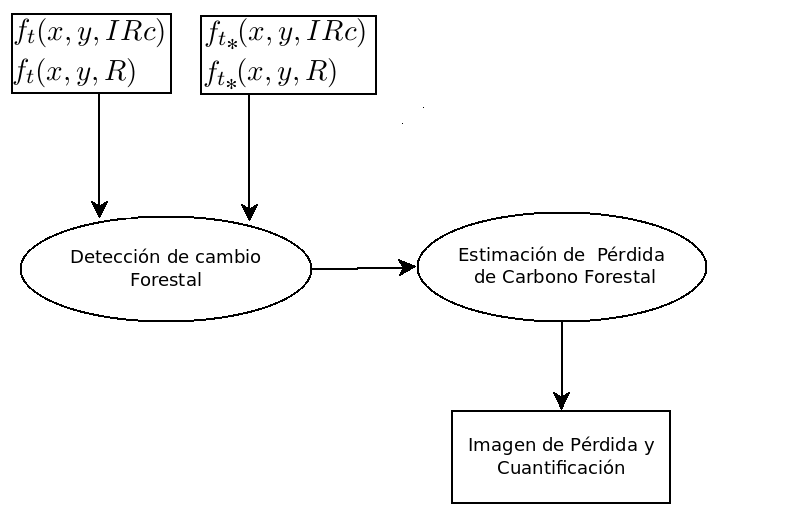
\includegraphics[width=1.0	\textwidth]{./Figures/cap4/metodologiaCarbono_3.png}
	\caption{Diagrama de flujo. Metodolog\'ia propuesta}
	\label{fig:metodologiapc}
\end{figure}

\subsection{Detecci\'on de cambio Forestal}
La detecci\'on de cambio cumple un papel fundamental en la metodolog\'ia ya que nos permite categorizar el cambio en la secuencia temporal estudiada. Este proceso presenta una metodolog\'ia automatizada a trav\'es del calculo de par\'ametros estad\'isticos extra\'ido de las im\'agenes satelitales y el uso de variables determinadas en un previo an\'alisis del comportamiento espectral observados en la cobertura vegetal de prueba.

\subsubsection{Detecci\'on de cambio}
En este proceso se detecta el cambio entre dos tiempos de im\'agenes satelitales. El resultado esperado constituye una mascara de cambio ($ MC $) entre las series temporales de im\'agenes comparadas. 
\paragraph{Comparaci\'on Multitemporal}\mbox{}\\\mbox{}\\
El siguiente paso despu\'es de haber equiparado radiom\'etricamente (secci\'on \ref{sec:capNormalizacion}) las im\'agenes consiste en la comparaci\'on multitemporal, permitiendo obtener un indice de cambio (variable cuantitativa) en cada pixel resultante. El m\'etodo de diferencia de im\'agenes es utilizada debido a que el m\'etodo Ratio no se ajusta a una distribuci\'on normal, se asume que el cambio es reducido y por ende est\'an ubicados hacia los extremos del histograma de la imagen con los \'indices de cambio $ I_{c} $, condici\'on clave para la umbralizaci\'on estad\'istica. La comparaci\'on es realizado sobre la imagen con los NDVI de cada serie temporal a modo a resaltar la vegetaci\'on y simplificar la cantidad de bandas utilizadas, observando a su vez que los datos estables ser\'an pr\'oximos a $ 0 $ gracias a la semejanza existente entre los pixeles. 
\paragraph{Umbral estad\'istico}\mbox{}\\\mbox{}\\
Los criterios de decisi\'on propuesto en la secci\'on \ref{sec:discriminacion} asignan valores de cambio/no cambio en funci\'on a un umbral. Estos criterios permiten convertir los indices de cambios a valores cualitativos que representan una m\'ascara de cambio ($ MC $). El m\'etodo basados en par\'ametros estad\'isticos es escogido por su sencillez y coherencia con el m\'etodo de comparaci\'on multitemporal aplicada. \\~\\
La imagen es re-clasificadas en distintas categor\'ias mediante los umbrales calculados (Perdida=2, Ganancia=1, No cambio=3), como podemos ver en la Figura \ref{fig:umbrales}.  La variable de fiabilidad $ n $ es elegida en base a la probabilidad de cambio deseado para la detecci\'on (m\'as detalles en la secci\'on \ref{sec:discriminacion}).
	\begin{figure}[H]
		\centering
		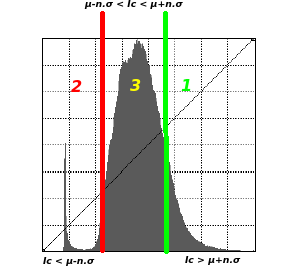
\includegraphics[width=0.5	\textwidth]{./Figures/cap4/umbrales.png}
		\caption{Umbrales y valores cualitativas asignadas en cada categor\'ia (Perdida=2, Ganancia=1, No cambio=3).}
		\label{fig:umbrales}
	\end{figure}

\paragraph{Iteraci\'on}\label{subsec:iteracion}\mbox{}\\\mbox{}\\
 Si dos im\'agenes se consideran semejantes, los cambios producidos en el terreno afectan a la radiometr\'ia registrada en las im\'agenes, y por tanto, en los par\'ametros estad\'isticos que las definen.\\~\\
En la normalizaci\'on radiom\'etrica los cambios introducen ruido \cite{martinez2013normalizacion}, ya que el proceso busca que los pixeles de una banda de im\'agenes satelitales en diferentes tiempos sean semejantes y el cambio estar\'ia influyendo en la correlaci\'on entre los pixeles que verdaderamente no sufrieron cambio. Si el \'area de todos los pixeles con cambio es mayor, la influencia en la normalizaci\'on ser\'a mayor y por ende afectara la precisi\'on en la detecci\'on de cambios. En vista al problema, mediante una normalizaci\'on radiom\'etrica iterativa se pretende minimizar dicha influencia, donde los par\'ametros estad\'isticos ($ \mu,\sigma $) utilizados constituyen los pixeles sin cambios.\\~\\
En la Figura \ref{fig:iteracionRadiometrica} podemos observar que a partir de la mascara de cambio obtenido en la primera iteraci\'on, los par\'ametros estad\'isticos para la iteracion 2, en la normalizaci\'on iterativa, son realizados sobre los pixeles que no detectaron cambios. 
	\begin{figure}[H]
		\centering
		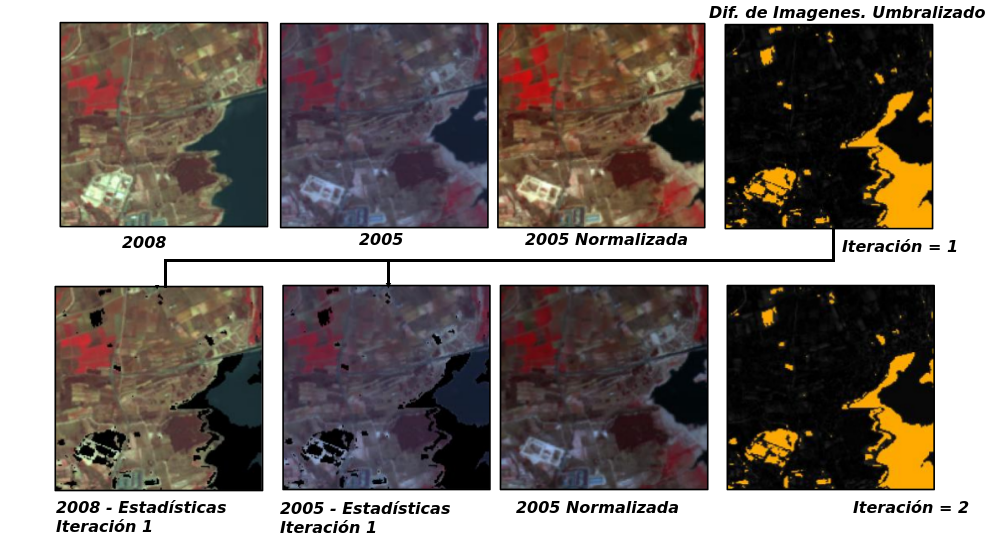
\includegraphics[width=1.0	\textwidth, height=0.5 \textheight]{./Figures/cap4/iteracionUmbra.png}
		\caption{Mascaras de cambio, iteraci\'on de la normalizaci\'on radiom\'etrica.}
		\label{fig:iteracionRadiometrica}
	\end{figure}
	
La Figura \ref{fig:deteccionCambio} nos presenta el ciclo de procedimientos para la detecci\'on de cambio, donde a partir de la secuencia de im\'agenes satelitales en las bandas infrarroja cercana y roja ($ f_{t}(x,y,IRc);f_{t}(x,y,R), f_{t_{*}}(x,y,IRc);f_{t*}(x,y,R) $) son calculados los par\'ametros estad\'isticos para las im\'agenes. Esos par\'ametros son utilizados para normalizan radiom\'etricamente las bandas del tiempo $ t_{*} $, en semejanza a las bandas de la imagen satelital del tiempo $ t $, as\'i determinar la imagen con los \'indices de cambios ($ I_{c} $) una vez hallados los NDVI ($ ndvi_{t},ndvi_{t_{*}} $). La mascara de cambio ($ MC $) es el resultado de pasar por los umbrales estad\'isticos. La imagen $ MC $ es binarizada tal que, los niveles digitales $ MC(x,y) = 2; MC(x,y) = 1 $ sean iguales a $ 0 $ y $ MC(x,y) = 3$ sean iguales a $ 1 $, de manera a discriminar solo los pixeles sin cambio ($ MC(x,y)=1 $). La iteraci\'on ($ iter $) continua si la media del $ I_{c}[iter] $ es de magnitud similar a la registrada en la anterior $  I_{c}[iter-1] $ o si $ iter=0 $, sino, el proceso es repetido pero con la variante que los par\'ametros estad\'isticos para la normalizaci\'on es calculado teniendo en cuenta solo aquellos pixeles que no sufrieron cambio.
\begin{figure}[H]
	\centering
	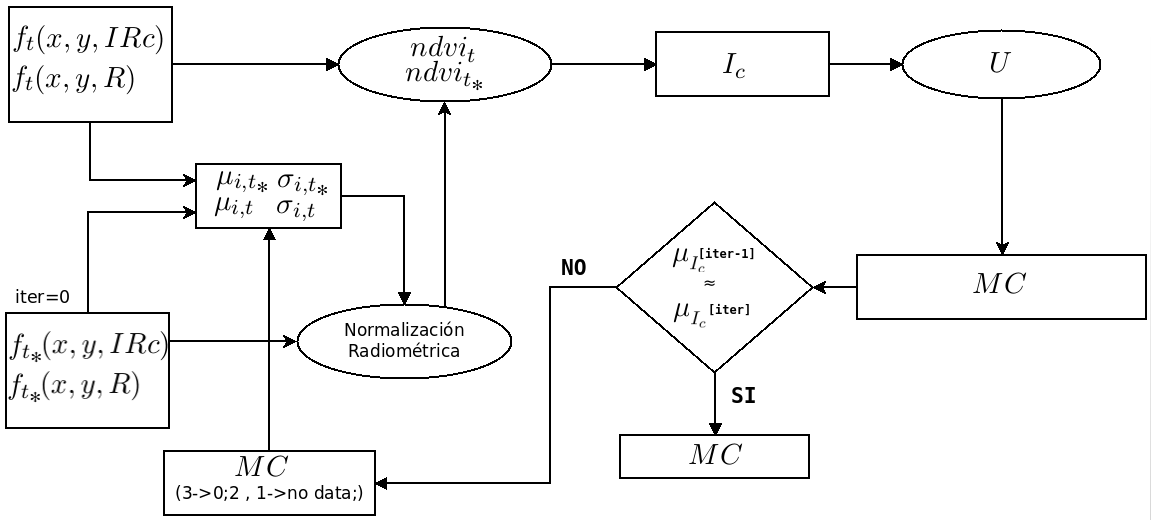
\includegraphics[width=1.0 \textwidth]{./Figures/cap4/deteccionCambio_3.png}
	\caption{Diagrama de flujo. Detecci\'on de Cambio.}
	\label{fig:deteccionCambio}
\end{figure}

\subsubsection{Discriminaci\'on Forestal}
Las im\'agenes procesadas son aquellas obtenidas en la ultima normalizaci\'on radiom\'etrica, generada por el proceso iterativo y la imagen base para la semejanza en ese proceso. En este procedimiento se busca generar una mascara de vegetaci\'on (MV) de la secuencia temporal.
\paragraph{NDVI}\mbox{}\\\mbox{}\\
El NDVI es calculado para ambas fechas pertenecientes a la serie temporal evaluada. El calculo es hecho teniendo como entradas las bandas infrarroja cercana y roja, donde el vigor vegetal de cada p\'ixel sera determinado por la ecuaci\'on \ref{e:ndvi}. En total son consumidas 4 im\'agenes para obtener dos de salidas.
\paragraph{Umbral de Vegetaci\'on}\label{sec:uvegetacion}\mbox{}\\\mbox{}\\
El umbral que discrimina la vegetaci\'on es determinado a partir de una constante calculada por un previo an\'alisis del comportamiento espectral de la cobertura vegetal y las im\'agenes de NDVI. Dicha variable corresponde a la desviaci\'on $(\sigma_{c} = 0.0658242733)  $ observada en la intersecci\'on entre im\'agenes VCF y Landsat (m\'as detalles en la secci\'on \ref{subsec:umbralVegetacion}). La ecuaci\'on del umbral $ U_{NDVI} $ tiene la siguiente expresi\'on:
		\begin{equation}
		U_{NDVI} = \mu_{NDVI}\pm n \times \sigma_{c}
		\end{equation}
\nomenclature[58]{$ \sigma_{c} $}{Desviaci\'on determinada como constante para la umbralizaci\'on de la cobertura vegetal.}
Donde $ \mu_{NDVI} $ representa la media del NDVI calculada y $ n $ la fiabilidad. La ecuaci\'on correspondiente a la suma no es utilizada debido a que se pretende incluir \'indices por debajo de la media. En la Figura \ref{fig:ndviUmbral} podemos observar que el umbral del NDVI se situ\'a por debajo de la media.
\begin{figure}[H]
	\centering
	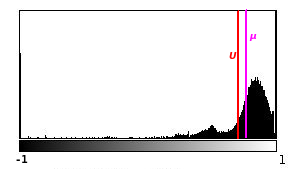
\includegraphics[width=0.8	\textwidth]{./Figures/cap4/ndviUmbral.png}
	\caption{Umbral NDVI y la media en el histograma de la imagen con NDVI.}
	\label{fig:ndviUmbral}
\end{figure}

\paragraph{Intersecci\'on \'area boscosa }\mbox{}\\\mbox{}\\
El procedimiento que sigue una vez obtenido los NDVI de las dos fechas es determinar los pixeles que ser\'an evaluados para detectar el cambio, por ello aplicamos una simple operaci\'on de uni\'on ($ ndvi_{1} $ OR $ ndvi_{2}$) que generara una mascara de vegetaci\'on $ MV $ correspondiente a los dos tiempos. La Figura \ref{fig:discrimForestal} refleja los pasos realizados para obtener una mascara de vegetaci\'on.
\begin{figure}[H]
	\centering
	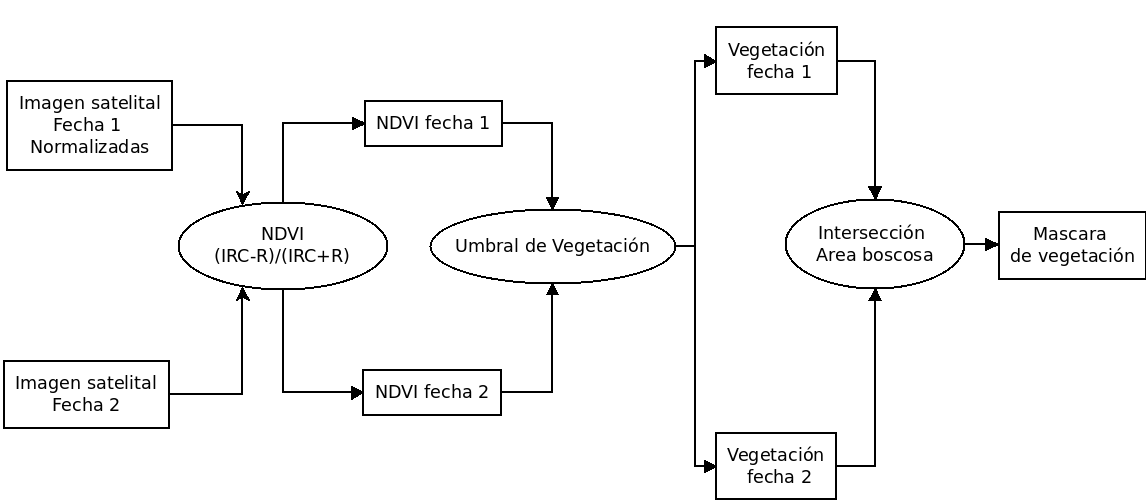
\includegraphics[width=1.0	\textwidth]{./Figures/cap4/discriminacionForestal_2.png}
	\caption{Diagrama de flujo. Discriminaci\'on Forestal.}
	\label{fig:discrimForestal}
\end{figure}


\subsubsection{Mascara de P\'erdida Forestal}
El proceso consiste en la intersecci\'on entre la mascaras de vegetaci\'on y cambio ($ MC$ AND $MV $). En la interseccion solo son considerados los cambios correspondiente a p\'erdidas en $ MC $, debido a que se pretende generar una imagen binaria $ MP $ que represente si en un pixel hay p\'erdida forestal.\\~\\
La imagen $ MP $ probablemente tendr\'a errores que son inherentes a los procesos utilizados para su creación \cite{lovell2001filtering}. \\~\\
La utilizaci\'on del filtro de mediana sobre la imagen de perdida en la reducci\'on del porcentaje de falsas alarmas ser\'a utilizado como m\'etodo para la eliminaci\'on de ruido. Con im\'agenes de media/alta resoluci\'on espacial(menos de $ 15 \times 15 $ metros cuadrados) se obtienen buenos resultados aplicando filtros de $ 5x5 $, pero cuando se trabaje con im\'agenes de menor resoluci\'on no se recomienda ese tama\~{n}o de ventana por la distorsi\'on que causa a la imagen \cite{martinez2013normalizacion}. Nuestras im\'agenes satelitales de entrada son de baja resoluci\'on espacial ($ 30 \times 30 $ metros cuadrados) por lo que el tama\~{n}o de ventana a utilizar seria $ 3 \times 3 $.
En la Figura \ref{fig:intersPerdida} podemos observar el flujo de tareas para la obtenci\'on de la mascara que representa la perdida forestal en dos tiempos .
\begin{figure}[H]
	\centering
	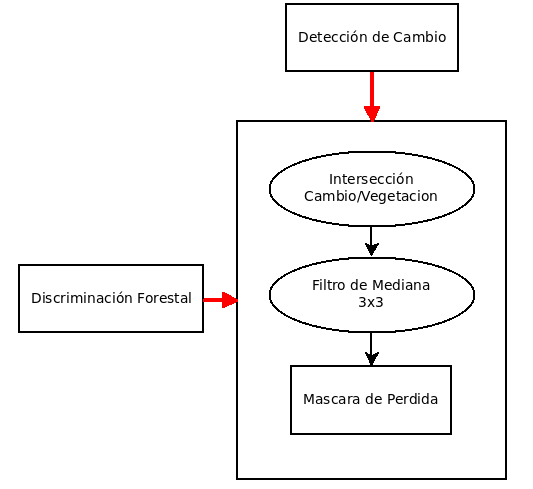
\includegraphics[width=0.8	\textwidth]{./Figures/cap4/interseccionPerdida.png}
	\caption{Diagrama de procedimientos para la obtenci\'on de la m\'ascara de perdida forestal.}
	\label{fig:intersPerdida}
\end{figure}

\subsection{Estimaci\'on de p\'erdida de carbono forestal}
El procedimiento final en la metodolog\'ia consiste en estimar el carbono perdido o no secuestrados dentro del tiempo transcurrido entre las im\'agenes satelitales. El producto constituye la mascara de perdida forestal junto con la cuantificaci\'on en toneladas de carbono por hect\'area obtenida mediante la ecuaci\'on de regresi\'on lineal $(y= b + a \times x) $. La ecuaci\'on de regresi\'on fue generada a trav\'es del mapa global de carbono \cite{saatchi2011benchmark} y el NDVI, determinadas por las im\'agenes Landsat, en un an\'alisis previo (m\'as detalles en la secci\'on \ref{subsec:estimacionCarbono}). La regresi\'on presenta un coeficiente de determinaci\'on moderado $ (r^{2}=0.509125) $, seg\'un la tabla \ref{t:coefDeter}, por lo que es considerada su aplicaci\'on en la metodolog\'ia.
\nomenclature[59]{$ r^{2}$}{Coeficiente de determinaci\'on.}
\begin{table}[H]
	\centering
	\begin{tabular}{|l|l|}
		\hline
		\textbf{Valor} & \textbf{Significado} \\ \hline
		0,0            & Ninguna Relaci\'on     \\ \hline
		0,25           & Relaci\'on baja        \\ \hline
		0,50           & Relaci\'on Moderada    \\ \hline
		0,75           & Relaci\'on Buena       \\ \hline
		1,00           & Relaci\'on perfecta    \\ \hline
	\end{tabular}
	\caption{Rangos del coeficiente de determinaci\'on.}
	\label{t:coefDeter}
\end{table}
Sea $ C:(x,y) \longrightarrow \{ [-\infty,\infty]\}$ la cantidad de carbono, en toneladas por hect\'area, para la coordenada $ (x,y) $, se tiene que: 

		\begin{equation}
			C(x,y)=4,33+30,1 \times ndvi(x,y)
		\end{equation}
		\nomenclature[60]{$ C(x,y)$}{Toneladas de carbono por hect\'area en las coordenadas $ (x,y) $.}

La estimaci\'on de carbono para dos fechas en funci\'on al ndvi ($ ndvi_{t},ndvi_{t_{*}} $) queda definida de la siguiente manera:
		\begin{equation}
		\label{e:fecha1}
		C_{t}(x,y)=4,33+30,1 \times ndvi_{t}(x,y)
		\end{equation}
		\begin{equation}
		\label{e:fecha2}
		C_{t_{*}}(x,y)=4,33+30,1 \times ndvi_{t_{*}}(x,y)
		\end{equation}
El c\'alculo de perdida de carbono en las fechas consistir\'ia b\'asicamente en $\Sigma^{m}_{x=0}\Sigma^{n}_{y=0} C_{t_{*}}(x,y) - \Sigma^{m}_{x=0}\Sigma^{n}_{y=0} C_{t}(x,y) $. El indice de cambio generado para la detecci\'on de cambio simplificar\'ia los c\'alculos ya que:
		\begin{equation}
		\label{e:indiceCambio}
		Ic(x,y)=ndvi_{t_{*}}(x,y) -ndvi_{t}(x,y)
		\end{equation}		

Podr\'iamos restar la ecuaci\'on \ref{e:fecha2} y \ref{e:fecha1}, tendr\'iamos:
		\begin{equation}
		\label{e:restaCar}
		C_{t_{*}}(x,y) - C_{t}(x,y)= 30,1 \times (ndvi_{t_{*}}(x,y)-ndvi_{t}(x,y))
		\end{equation}		
		\begin{equation}
		\label{e:perdidaCar}
		PC(x,y)= C_{t_{*}}(x,y) - C_{t}(x,y)
		\end{equation}		
		\nomenclature[62]{$Ic(x,y)$}{ Indice de cambio en las coordenadas $ (x,y) $.}
		\nomenclature[63]{$PC(x,y)$}{Toneladas de carbono por hect\'area perdidos en las coordenadas $ (x,y) $.}
		
Siendo $ PC(x,y)$ toneladas de carbono por hect\'area perdidos. Remplazando \ref{e:indiceCambio} y \ref{e:perdidaCar} en \ref{e:restaCar}, la ecuaci\'on de regresi\'on final quedar\'ia:
\begin{equation}\label{ec:carbono}
PC(x,y) = 30,1 \times Ic(x,y)
\end{equation}
La ecuaci\'on \ref{ec:carbono} debe ser multiplicada por un factor de $ 0,09 $, debido a que los pixeles del mapa global de carbono representan toneladas de carbono por hect\'area \cite{saatchi2011benchmark} y la superficie m\'inima representada por las imagenes Landsat (utilizadas para el calculo de NDVI) es de $ 900m^{2}=0.09 toneladas $. La ecuaci\'on final quedar\'ia:
\begin{equation}\label{ec:carbonoFinal}
PC(x,y) = 2.709 \times Ic(x,y)
\end{equation}
La cuantificaci\'on sera realizado teniendo en cuenta la mascara de perdida forestal. La Figura \ref{fig:resulPC} nos muestra el resultado esperado por la metodolog\'ia (Mascara de perdida Forestal y cuantificaci\'on).
\begin{figure}[H]
	\centering
	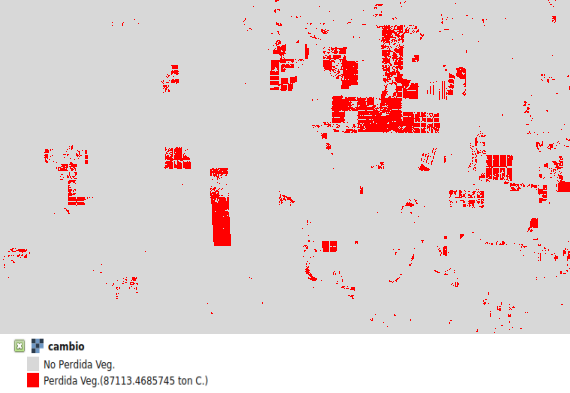
\includegraphics[width=0.8	\textwidth]{./Figures/cap4/resultadoMetodologia.png}
	\caption{Presentaci\'on del resultado. Mascara de perdida Forestal y cuantificaci\'on.}
	\label{fig:resulPC}
\end{figure}
\section{Resumen}
En este capitulo se describen los materiales y los tres procedimientos generales que componen la metodolog\'ia propuesta. La im\'agenes infrarroja cercana y roja de las dos fechas inicialmente deben pasar por un proceso de correcci\'on de errores del sensor y de ubicaci\'on geogr\'afica para realizar el an\'alisis multitemporal en la detecci\'on de cambio forestal. Una vez detectado la perdida forestal entre las fechas del proceso de detecci\'on de cambio, se realiza la estimaci\'on de carbono en base a una ecuaci\'on de regresi\'on hallado por un estudio previo. El resultado consiste en un mapa de perdida forestal junto a la cuantificaci\'on en toneladas de carbono perdidos.